% Template for the validation preprint. Do not edit numbers here: tokens like 88.4
% are filled from paper/stats.json by code/10_preprint_tex.py, which writes paper/preprint/main.tex.
\documentclass[aps,prd,reprint,superscriptaddress,amsmath,amssymb,floatfix,nofootinbib]{revtex4-2}
\usepackage{graphicx}
\usepackage{xcolor}
\definecolor{linkblue}{RGB}{28,92,171}
\usepackage[colorlinks=true,linkcolor=red!70!black,citecolor=red!70!black,urlcolor=linkblue]{hyperref}
\usepackage{orcidlink}

\begin{document}

\title{How Rural Is Rural? Agreement Between the FARS Rural/Urban Label and 2020 Census Urban Areas for U.S.\ Traffic Deaths, 2015--2024}

\author{Emmanuel Oti Nani\,\orcidlink{0009-0009-4175-8962}}
\email{otiemmanuelnani@gmail.com}
\affiliation{Independent Researcher, Springfield, Missouri, USA}

\begin{abstract}
U.S. rural road safety statistics, including the National Highway Traffic Safety Administration's annual rural/urban fatality reports, classify each fatal crash by the rural/urban variable (RUR\_URB) in the Fatality Analysis Reporting System (FARS). Population research, in contrast, usually defines rural with the Census Bureau's urban areas. We measure how well the two definitions agree for every fatal crash with a usable location from 2015 to 2024 (355{,}591 crashes, 386{,}140 deaths), placing each crash on the 2020 Census urban-area map, held fixed across years, and comparing the result with its FARS label. The two definitions agree on 88.4\% of deaths (Cohen's $\kappa = 0.77$). Disagreement runs mainly in one direction: 17.5\% of deaths in crashes outside Census urban areas carry an urban FARS label, against 5.8\% in the opposite direction. These crashes cluster at urban edges, with a median distance of 0.65~km to the nearest Census urban area, compared with 9.76~km for crashes that both definitions call rural. The gap widened over the decade. The FARS rural share of deaths fell from 50.1\% in 2015 to 41.1\% in 2024, while the fixed-map share moved from 52.0\% to 48.1\%. The divergence is concentrated in a few states and, in New York and California, appears as a single step between 2017 and 2018. Rural road safety trends based on the FARS label therefore mix changes in where crashes occur with changes in how they are labeled. Analyses should state their rural definition and, for trends, hold it fixed. The county panel, crash-level crosswalk, and code are openly available.
\\[4pt]
\textbf{Keywords:} rural roads, traffic fatalities, FARS, urban areas, measurement validity, road safety data
\end{abstract}

\maketitle

\section{Introduction}

Rural roads carry a share of U.S.\ traffic deaths far larger than the rural share of the population. Of 39{,}254 traffic fatalities in 2024, the National Highway Traffic Safety Administration (NHTSA) reports that 16{,}006 (41\%) occurred in rural areas, where about 21\% of Americans live~\cite{nhtsa2026ru}. Studies of the rural excess have long attributed it to higher fatality rates per crash, longer emergency response, higher speeds, and lower restraint use~\cite{zwerling2005,peekasa2004}. Such comparisons depend on what counts as rural, and federal agencies do not use one definition~\cite{hart2005,ratcliffe2016}.

National crash statistics classify each fatal crash with the FARS data element RUR\_URB. It records whether the trafficway segment lies inside or outside urban boundaries that state transportation agencies adjust from the Census Bureau's urban areas and that the Federal Highway Administration (FHWA) approves~\cite{farsmanual2026,fhwa2023}. Population counts, including the statement that one American in five lives in a rural area, use the Census urban areas themselves~\cite{ratcliffe2016}. When the rural share of deaths from one definition is set against the rural share of population from the other, the comparison is only as sound as the agreement between the two. For the 2020 Census, the Census Bureau also revised its urban-area criteria, raising the minimum size of an urban area to 2{,}000 housing units or 5{,}000 people~\cite{census2022criteria,census2022final}. Highway agencies then updated their adjusted boundaries on their own schedules.

This paper asks three questions. How often do the FARS rural/urban label and the 2020 Census urban-area map agree for U.S.\ traffic deaths? When they disagree, in which direction, and where? Does the agreement change between 2015 and 2024, enough to alter the apparent trend in rural deaths? The analysis is part of an open county-by-year panel of FARS deaths that holds the rural definition fixed, released with a crash-level crosswalk so that others can reproduce or extend it~\cite{panel2026}. Section~\ref{sec:data} describes the data and the two definitions, Sec.~\ref{sec:methods} the agreement measures, Sec.~\ref{sec:results} the results, and Sec.~\ref{sec:discussion} their implications and limits.

\section{Data and definitions}\label{sec:data}

\subsection{Fatal crashes}

FARS is NHTSA's census of crashes on U.S.\ public roads in which a person dies within 30 days. We used the national FARS files for 2015--2024~\cite{farsdata}: Final Files for 2015--2023 and the Annual Report File for 2024, first released on April 1, 2026. The accident file gives each crash's state and county codes, latitude and longitude, RUR\_URB, functional system (FUNC\_SYS), and number of deaths (FATALS). The files contain 358{,}460 crashes and 389{,}190 deaths. In every year, the FATALS total equals the number of persons with a fatal injury (INJ\_SEV $=4$) in the person file, and the 2024 total matches NHTSA's published figure~\cite{nhtsa2026ru}.

\subsection{Reference definition: 2020 Census urban areas}

A crash is classed \emph{urban} when its coordinates fall inside a 2020 Census urban area~\cite{census2022final,tiger} and \emph{rural} otherwise. The same 2020 map is applied to every year, so a change in the rural share over time reflects where crashes occurred, not a change in boundaries. Coordinates are usable when latitude lies between 17$^\circ$ and 72$^\circ$ N, longitude between 64$^\circ$ and 180$^\circ$ W (which excludes the FARS missing-value codes 77.7777, 88.8888, and 99.9999), and the point falls inside a U.S.\ county.

\subsection{Comparison definition: the FARS label}

RUR\_URB ``identifies the classification of the segment of the trafficway on which the crash occurred based on FHWA-approved adjusted Census boundaries of small urban and urbanized areas''~\cite{farsmanual2026}. Code 1 is rural and code 2 urban. Codes 6 (trafficway not in state inventory), 8 (not reported), and 9 (unknown) were treated as unknown. NHTSA reintroduced the element in 2015 after a period in which rural and urban were derived from the roadway function class~\cite{farsmanual2026}, which is why the analysis begins in 2015.

\subsection{Analytic sample}

A crash enters the comparison when it has usable coordinates and a known FARS label. Of 358{,}460 crashes, 355{,}591 (99.2\%) qualify, with 386{,}140 deaths; 2{,}869 are excluded. Every crash is also linked to its 2020 county, place, and county subdivision in the published crosswalk~\cite{panel2026}.

\section{Methods}\label{sec:methods}

For each comparison we form a two-by-two table with cells $a$ (rural under both definitions), $b$ (rural on the Census map, urban in FARS), $c$ (urban on the Census map, rural in FARS), and $d$ (urban under both), weighted by deaths, the unit of rural/urban fatality reporting, with $N=a+b+c+d$. Observed agreement and the agreement expected by chance are
\begin{equation}
p_o = \frac{a+d}{N},
\end{equation}
\begin{equation}
p_e = \frac{(a+b)(a+c)+(c+d)(b+d)}{N^2},
\end{equation}
and Cohen's kappa is~\cite{cohen1960}
\begin{equation}
\kappa = \frac{p_o - p_e}{1 - p_e}.
\end{equation}
Taking the Census map as the reference, the share of Census-rural deaths that FARS labels rural ($S_e$) and the share of Census-urban deaths that FARS labels urban ($S_p$) are
\begin{equation}
S_e = \frac{a}{a+b}, \qquad S_p = \frac{d}{c+d}.
\end{equation}
The rural share of deaths under each definition is
\begin{equation}
R_{\mathrm{Census}} = \frac{a+b}{N}, \qquad R_{\mathrm{FARS}} = \frac{a+c}{N},
\end{equation}
so the gap between them, $R_{\mathrm{Census}}-R_{\mathrm{FARS}} = (b-c)/N$, is the net of the two kinds of disagreement.

Neither definition is ground truth; they serve different purposes. $S_e$ and $S_p$ are therefore measures of correspondence with the Census definition, not of accuracy. We report the measures overall, by year, for 2015--2019 and 2020--2024, by FARS road class, and by state. To locate disagreements, we computed for each Census-rural crash the distance from its coordinates to the nearest 2020 Census urban area (Albers equal-area projection) and compared crashes labeled urban and rural by FARS. To find where the trend diverges, we compared each state's change in rural share between 2015--2016 and 2023--2024 under the two definitions. As a sensitivity check, all measures were recomputed with crashes instead of deaths as the unit. Analyses used Python with GeoPandas; the code is in the replication package~\cite{panel2026}.

\section{Results}\label{sec:results}

\subsection{Overall agreement}

Table~\ref{tab:twobytwo} gives the 2015--2024 cross-classification. The definitions agree on 88.4\% of 386{,}140 deaths, with $\kappa = 0.768$, in the range conventionally called substantial~\cite{landis1977}. Disagreement is asymmetric. Of deaths outside Census urban areas, 82.5\% carry a rural FARS label and 17.5\% (33{,}505 deaths) an urban one. Of deaths inside Census urban areas, 94.2\% carry an urban label and 11{,}208 deaths a rural one. As a result, 49.5\% of compared deaths are rural on the Census map and 43.7\% under the FARS label. Weighting by crashes instead of deaths changes little: agreement 88.5\%, $\kappa = 0.768$, $S_e = 82.2$\%.

\begin{table}[t]
\caption{Cross-classification of deaths by the 2020 Census urban-area map and the FARS rural/urban label, 2015--2024.}
\label{tab:twobytwo}
\begin{ruledtabular}
\begin{tabular}{lrrr}
 & FARS rural & FARS urban & Total \\
\hline
Census map rural & 157{,}684 & 33{,}505 & 191{,}189 \\
Census map urban & 11{,}208 & 183{,}743 & 194{,}951 \\
Total & 168{,}892 & 217{,}248 & 386{,}140 \\
\end{tabular}
\end{ruledtabular}
\end{table}

\subsection{Change over time}

Table~\ref{tab:years} and Fig.~\ref{fig:share} show the comparison by year. The FARS rural share fell from 50.1\% in 2015 to 41.1\% in 2024, a decline of 9.0 percentage points. Under the fixed Census map, the rural share fell from 52.0\% to 48.1\%, a decline of 3.9 points. The gap between the definitions widened from 1.9 to 6.9 points. The share of Census-rural deaths labeled rural by FARS fell from 85.7\% to 80.8\%, and the share of Census-urban deaths labeled urban rose from 88.4\% to 95.6\%, so the FARS label moved toward urban in both cells. Overall agreement did not fall ($\kappa = 0.751$ in 2015--2019 and 0.783 in 2020--2024) because the urban-direction changes offset each other in $p_o$. In counts, deaths in crashes outside Census urban areas went from 18{,}325 in 2015 to 18{,}760 in 2024, while deaths with a rural FARS label went from 17{,}715 to 16{,}005.

\begin{table*}[t]
\caption{Agreement between the FARS rural/urban label and 2020 Census urban areas by crash year, deaths with a known location under both definitions. $S_e$: share of Census-rural deaths labeled rural by FARS. $S_p$: share of Census-urban deaths labeled urban by FARS.}
\label{tab:years}
\begin{ruledtabular}
\begin{tabular}{lrrrrrrr}
Year & Deaths & Agreement (\%) & $\kappa$ & $S_e$ (\%) & $S_p$ (\%) & Rural, Census map (\%) & Rural, FARS label (\%) \\
\hline
2015 & 35{,}136 & 87.0 & 0.739 & 85.7 & 88.4 & 52.0 & 50.1 \\
2016 & 37{,}545 & 87.9 & 0.759 & 85.5 & 90.5 & 51.4 & 48.6 \\
2017 & 37{,}205 & 87.2 & 0.744 & 83.0 & 91.4 & 50.9 & 46.5 \\
2018 & 36{,}514 & 87.4 & 0.749 & 80.8 & 94.2 & 50.5 & 43.6 \\
2019 & 36{,}176 & 88.2 & 0.765 & 82.6 & 94.0 & 50.8 & 44.9 \\
2020 & 38{,}698 & 89.5 & 0.788 & 82.1 & 96.6 & 49.0 & 42.0 \\
2021 & 42{,}989 & 90.0 & 0.799 & 81.7 & 97.6 & 47.7 & 40.2 \\
2022 & 42{,}391 & 89.0 & 0.778 & 81.1 & 96.3 & 47.9 & 40.8 \\
2023 & 40{,}722 & 89.0 & 0.777 & 81.5 & 95.8 & 47.8 & 41.1 \\
2024 & 38{,}764 & 88.5 & 0.769 & 80.8 & 95.6 & 48.1 & 41.1 \\
\end{tabular}
\end{ruledtabular}
\end{table*}

\begin{figure}[t]
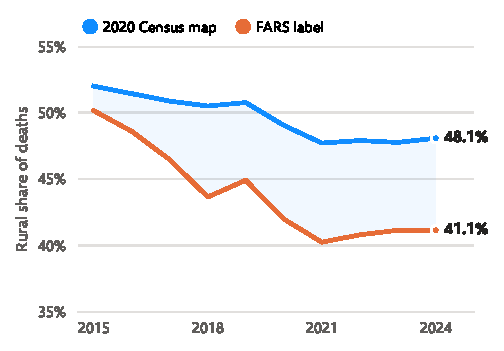
\includegraphics[width=\columnwidth]{fig1_rural_share.pdf}
\caption{Rural share of deaths by crash year under the 2020 Census urban-area map (held fixed) and the FARS RUR\_URB label. Deaths with a known location under both definitions.}
\label{fig:share}
\end{figure}

\subsection{Where the definitions disagree}

Deaths outside Census urban areas that FARS labels urban lie close to urban areas (Fig.~\ref{fig:distance}). Their median distance to the nearest 2020 Census urban area is 0.65~km, and 58.6\% lie within 1~km and 87.2\% within 5~km. For deaths that both definitions class as rural, the median distance is 9.76~km, with 7.4\% within 1~km and 29.8\% within 5~km. The urban-labeled cases are therefore concentrated in the fringe immediately around Census urban areas.

\begin{figure}[t]
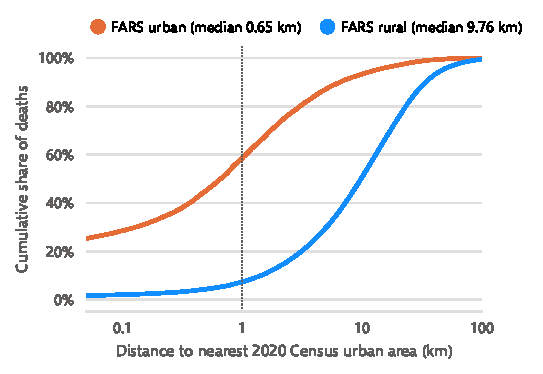
\includegraphics[width=\columnwidth]{fig2_distance_ecdf.pdf}
\caption{Cumulative distribution of the distance from crash location to the nearest 2020 Census urban area, for deaths outside Census urban areas, by FARS label, 2015--2024. Weighted by deaths; logarithmic horizontal axis. The dotted line marks 1~km.}
\label{fig:distance}
\end{figure}

Agreement varies little across road classes (Table~\ref{tab:road}). It is lowest on Interstates and other freeways, where $S_e$ is also lowest, and highest on collectors. Among states with at least 500 compared deaths in 2022--2024, agreement ranges from 82.2\% (West Virginia) to 96.0\% (Nebraska).

\begin{table}[t]
\caption{Agreement by FARS road class (FUNC\_SYS), deaths, 2015--2024. Arterial: other principal and minor arterials; collector: major and minor collectors.}
\label{tab:road}
\begin{ruledtabular}
\begin{tabular}{lrrrrr}
Road class & Deaths & Agr.\ (\%) & $\kappa$ & $S_e$ (\%) & $S_p$ (\%) \\
\hline
Interstate, freeway & 67{,}015 & 86.4 & 0.714 & 75.6 & 94.1 \\
Arterial & 200{,}574 & 88.8 & 0.767 & 79.8 & 95.6 \\
Collector & 72{,}493 & 89.7 & 0.761 & 88.4 & 93.1 \\
Local & 45{,}405 & 87.8 & 0.756 & 87.2 & 88.6 \\
\end{tabular}
\end{ruledtabular}
\end{table}

\subsection{State patterns over time}

The widening national gap is not spread evenly. Comparing 2015--2016 with 2023--2024, the FARS rural share fell at least 5 points more than the Census-map share in 16 states, and rose at least 5 points more in 2 (Table~\ref{tab:states}). Among the 28 states with at least 2{,}000 deaths in those years, 10 show such a divergence. In New York and California, the FARS rural share dropped in one step between 2017 and 2018, from 45.3\% to 27.1\% and from 36.7\% to 28.6\%, while the Census-map share stayed nearly flat (Fig.~\ref{fig:states}). A one-year step of that size is unlikely to reflect where crashes occurred.

\begin{table}[t]
\caption{Rural share of deaths (\%) in 2015--2016 and 2023--2024 under each definition, for states with at least 2{,}000 deaths in those years: the six with the largest decline in the FARS share relative to the Census-map share, and the two with the largest relative rise. Divergence is the change in the FARS share minus the change in the Census-map share, in percentage points.}
\label{tab:states}
\begin{ruledtabular}
\begin{tabular}{lrrrrrr}
 & & \multicolumn{2}{c}{FARS label} & \multicolumn{2}{c}{Census map} & \\
State & Deaths & 15--16 & 23--24 & 15--16 & 23--24 & Div. \\
\hline
New York & 4{,}200 & 40.9 & 26.3 & 35.1 & 34.2 & -13.9 \\
California & 15{,}228 & 41.5 & 26.2 & 36.5 & 33.2 & -12.0 \\
Kentucky & 3{,}109 & 75.3 & 61.5 & 68.7 & 63.7 & -8.8 \\
Virginia & 3{,}328 & 63.6 & 50.9 & 61.0 & 56.7 & -8.4 \\
Michigan & 4{,}192 & 47.4 & 40.4 & 47.1 & 48.4 & -8.3 \\
Florida & 12{,}360 & 28.9 & 21.7 & 27.4 & 27.9 & -7.7 \\
\hline
New Jersey & 2{,}396 & 13.3 & 12.2 & 25.9 & 22.4 & +2.4 \\
Maryland & 2{,}206 & 22.9 & 19.3 & 38.8 & 30.4 & +4.7 \\
\end{tabular}
\end{ruledtabular}
\end{table}

\begin{figure}[t]
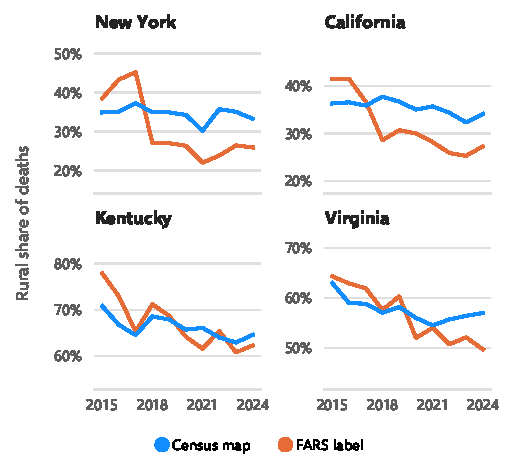
\includegraphics[width=\columnwidth]{fig3_state_series.pdf}
\caption{Rural share of deaths by year under the two definitions in the four states with at least 2{,}000 deaths in 2015--2016 and 2023--2024 and the largest divergence. Each panel has its own vertical scale.}
\label{fig:states}
\end{figure}

\section{Discussion}\label{sec:discussion}

The FARS rural/urban label and the 2020 Census urban-area map agree on most traffic deaths, but not at random. When they disagree, FARS usually labels a crash urban that the Census map places outside an urban area, and those crashes sit within about a kilometer of an urban area. This is consistent with how the label is built. RUR\_URB follows FHWA-approved adjusted urban boundaries~\cite{farsmanual2026}, which states draw around the Census urban areas for transportation planning and may extend to include adjacent development and road segments~\cite{fhwa2023}. The Census Bureau's 2020 criteria, by raising the minimum size of an urban area, also moved small places from urban to rural~\cite{census2022criteria}. Both features enlarge the area labeled urban by FARS relative to the Census map.

Two consequences follow. First, the FARS label yields a lower rural count. In 2024 the difference was 2{,}755 deaths nationally. Published comparisons that set the rural share of deaths from the FARS label against the rural share of population from the Census map mix the two definitions, and because the FARS label counts fewer rural deaths, those comparisons understate rather than overstate the rural excess. Second, and more consequential for trend analysis, the gap widened over the decade. Part of the reported decline in the rural share of deaths reflects a change in labeling rather than a shift in where crashes occur. The state results point to the same conclusion: the divergence is concentrated in a few states and, where it is largest, appears as a step change. This analysis cannot identify the cause of each step. Plausible causes include updates to adjusted urban boundaries between censuses and changes in how states link crash locations to their road inventories; confirming them requires state-level documentation.

The fixed-map series has its own limitation. Applying 2020 boundaries to 2015 crashes treats areas that urbanized during the decade as urban throughout, which understates the rural share early in the period. Some of its modest decline may therefore reflect the reverse problem. The two series bracket different definitional choices rather than one being correct.

For users of FARS, three practices follow. State the rural definition. For trends, hold the definition fixed, for example by geocoding crashes to one urban-area vintage, as the accompanying panel does~\cite{panel2026}. When computing rates, take deaths and population from the same definition.

\subsection{Limitations}

The reference standard is a definition, not ground truth. FARS coordinates can be imprecise, which matters most near urban-area edges, where most disagreements lie. About 0.8\% of crashes lacked usable coordinates or a known label and were excluded. The 2024 data are NHTSA's preliminary Annual Report File; small revisions are expected in the Final File. State estimates for small states are imprecise.

\section{Concluding remarks}

Across 386{,}140 deaths from 2015 to 2024, the FARS rural/urban label agrees with the 2020 Census urban-area map for most crashes ($\kappa = 0.77$) but systematically counts fewer rural deaths, mainly by labeling crashes at the edges of urban areas as urban. The gap grew between 2015 and 2024, unevenly across states and in steps in some. Rural road safety trends based on the FARS label should be read with this in mind, and analyses of rural trends should hold the rural definition fixed across years.

\section*{Data availability}

The county-by-year panel, the crash-level crosswalk to 2020 Census geography, the validation tables, and all code are openly available under CC BY 4.0 (data) and MIT (code) at Zenodo (DOI assigned at release) and \url{https://github.com/Emmanuel-Oti-Nani/rural-road-fatality-panel}. An interactive atlas is at \url{https://emmanuel-oti-nani.github.io/rural-road-fatality-panel/}.

\section*{Declarations}

\textbf{Funding.} None. \textbf{Competing interests.} None. \textbf{Ethics.} Analysis of public, de-identified federal data. \textbf{Use of AI tools.} Claude (Anthropic) assisted with code, data assembly, and drafting; the author designed the study, made the analytic decisions, verified the reported figures against the source files, and is responsible for the content.

\begin{thebibliography}{99}

\bibitem{nhtsa2026ru} National Highway Traffic Safety Administration. Traffic safety facts 2024 data: Rural/urban traffic fatalities. Report No.\ DOT HS 813 828, U.S.\ Department of Transportation, 2026. \url{https://crashstats.nhtsa.dot.gov/Api/Public/ViewPublication/813828}

\bibitem{zwerling2005} C. Zwerling, C. Peek-Asa, P. S. Whitten, S.-W. Choi, N. L. Sprince, and M. P. Jones. Fatal motor vehicle crashes in rural and urban areas: decomposing rates into contributing factors. \textit{Inj. Prev.}, 11(1):24--28, 2005. \href{https://doi.org/10.1136/ip.2004.005959}{doi:10.1136/ip.2004.005959}

\bibitem{peekasa2004} C. Peek-Asa, C. Zwerling, and L. Stallones. Acute traumatic injuries in rural populations. \textit{Am. J. Public Health}, 94(10):1689--1693, 2004. \href{https://doi.org/10.2105/AJPH.94.10.1689}{doi:10.2105/AJPH.94.10.1689}

\bibitem{hart2005} L. G. Hart, E. H. Larson, and D. M. Lishner. Rural definitions for health policy and research. \textit{Am. J. Public Health}, 95(7):1149--1155, 2005. \href{https://doi.org/10.2105/AJPH.2004.042432}{doi:10.2105/AJPH.2004.042432}

\bibitem{ratcliffe2016} M. Ratcliffe, C. Burd, K. Holder, and A. Fields. Defining rural at the U.S.\ Census Bureau. American Community Survey and Geography Brief ACSGEO-1, U.S.\ Census Bureau, 2016. \url{https://www.census.gov/library/publications/2016/acs/acsgeo-1.html}

\bibitem{farsmanual2026} National Center for Statistics and Analysis. Fatality Analysis Reporting System analytical user's manual, 1975--2024. Report No.\ DOT HS 813 794, National Highway Traffic Safety Administration, April 2026. \url{https://crashstats.nhtsa.dot.gov/Api/Public/ViewPublication/813794}

\bibitem{fhwa2023} Federal Highway Administration. Highway functional classification concepts, criteria and procedures, 2023 edition. U.S.\ Department of Transportation, 2023. \url{https://www.fhwa.dot.gov/policyinformation/hpms/hfcccp.cfm}

\bibitem{census2022criteria} U.S. Census Bureau. Urban area criteria for the 2020 Census---final criteria. \textit{Federal Register}, 87:16706, March 24, 2022.

\bibitem{census2022final} U.S. Census Bureau. 2020 Census qualifying urban areas and final criteria clarifications. \textit{Federal Register}, 87:80114--80154, December 29, 2022.

\bibitem{farsdata} National Highway Traffic Safety Administration. Fatality Analysis Reporting System, national data files 2015--2024 [data set]. \url{https://www.nhtsa.gov/file-downloads?p=nhtsa/downloads/FARS/}

\bibitem{tiger} U.S. Census Bureau. TIGER/Line shapefiles: 2020 urban areas (2023 vintage) and 2020 counties, places, and county subdivisions [data set]. \url{https://www.census.gov/geographies/mapping-files/time-series/geo/tiger-line-file.html}

\bibitem{cohen1960} J. Cohen. A coefficient of agreement for nominal scales. \textit{Educ. Psychol. Meas.}, 20(1):37--46, 1960. \href{https://doi.org/10.1177/001316446002000104}{doi:10.1177/001316446002000104}

\bibitem{landis1977} J. R. Landis and G. G. Koch. The measurement of observer agreement for categorical data. \textit{Biometrics}, 33(1):159--174, 1977. \href{https://doi.org/10.2307/2529310}{doi:10.2307/2529310}

\bibitem{panel2026} E. O. Nani. U.S. Rural Road Fatality County Panel, 2015--2024 (version 1.0.0) [data set and code]. Zenodo (DOI assigned at release); \url{https://github.com/Emmanuel-Oti-Nani/rural-road-fatality-panel}

\end{thebibliography}

\end{document}
